\documentclass[a4paper,11pt,spanish]{article}
\usepackage [spanish] {babel}
%\usepackage[utf8x]{inputenc}
\usepackage[T1]{fontenc}
\usepackage[spanish]{babel}

% Definici�n del formato
% Basic packages
\usepackage{graphicx}	% Needed to include figures in the document
\usepackage[body={0.6in, 8.2in},left=1.25in,right=1.25in]{geometry}
					% Geometry package for easy page margin
\usepackage{fancyhdr}
\usepackage[nottoc,notlof,notlot]{tocbibind}	% Show Bibliography in table of contents
\usepackage{listings}

\usepackage{color}

\usepackage{hyperref}

% Paragraph structure
\parindent=0.5cm
\parskip=5mm

% Document
\begin{document}

% P�gina de t��tulo
\title{\vskip 170pt
	TICO \\
	\Huge \bfseries \strut{Manual de usuario} \strut
	\vskip 30pt
}
\date{}

\maketitle

\thispagestyle{empty}
% Licencia
\newpage
\begin{flushright}
Este manual est� publicado bajo licencia \\
\textit{Creative Commons Attibution-NonCommercial-ShareAlike 2.5}. \\ 
Para m�s informaci�n, dirigirse a  \\
\texttt{http://creativecommons.org/licenses/by-nc-sa/2.5/es/}.
\end{flushright}

% �ndices
\newpage
\tableofcontents
\listoffigures

% Manual
\newpage
% Introducci�n
\section{Introducci�n}\label{sec:manual.introduccion}

\par Este es el manual de usuario de \textbf{TICO}, para su \textbf{versi�n 1.5}.
En �l se explica el funcionamiento de la aplicaci�n, su aspecto y las formas
de realizar cada una de las posibles acciones.

% Instalaci�n de la aplicaci�n
\section{Instalaci�n y ejecuci�n de la aplicaci�n}\label{sec:manual.instalacion}

\par La aplicaci�n se distribuye en dos ficheros diferentes, que corresponden con su instalaci�n
en diferentes sistemas operativos, y otro que corresponde con el c�digo fuente de la aplicaci�n.

\subsection{En Windows}\label{sec:manual.instalacion.windows}

\par Para instalar \texttt{TICO} en \textsl{Windows} hay que ejecutar el instalador que se distribuye con la aplicaci�n (\texttt{tico-bin-w32-e1.5.exe}) y seguir las instrucciones que ah� se indican.

\par El instalador crea autom�ticamente dos ejecutables, uno para el Editor y otro para el Int�rprete dentro de la carpeta de instalaci�n seleccionada. Tambi�n crea los accesos directos correspondientes en el \textsl{Escritorio} y el \textsl{Men� de inicio}. Como argumento de cualquiera de los dos ejecutables, se le puede pasar la direcci�n de un fichero de proyecto de \textbf{TICO} para que sea abierto nada m�s ejecutar la aplicaci�n.

\subsection{En otros sistemas operativos}\label{sec:manual.instalacion.otros}

\par Para instalar \textbf{TICO} en cualquier otro sistema operativo hay que
descomprimir el archivo comprimido \texttt{tico-bin-other-e1.5.zip} en la carpeta
elegida para ello.

\par Para ejecutar la aplicaci�n en otros sistemas operativos se proveen
dos ejecutables diferentes. Uno para sistemas operativos \textsl{Windows}
(\texttt{tico.bat}), por si alguien no quiere utilizar el instalador, y otro para sistemas operativos tipo \textsl{Unix} (\texttt{tico.sh}). Ambos ejecutables sirven tanto para el Int�rprete como para el Editor seg�n los argumentos con los que se invoquen. Para ejecutar el Int�rprete o el Editor hay que utilizar, como primer par�metro, la opciones \texttt{-i} y \texttt{-e} respectivamente, ejecut�ndose el Editor en caso de que no se utilice ninguna. Como segundo argumento se puede utilizar la direcci�n de un fichero de proyecto de \textbf{TICO}, que ser� abierto de inicio de la ejecuci�n de la aplicaci�n correspondiente.

\subsection{Aplicaciones requeridas}\label{sec:manual.instalacion.aplicaciones}

\par Para que la aplicaci�n se pueda ejecutar es necesario tener instalada, en el ordenador en el que se va a utilizar, una versi�n de la \textsl{M�quina Virtual de Java} igual o superior a la 1.6. Su descarga es gratuita y se puede realizar desde la
direcci�n web de \textsl{Sun Microsystems} o desde \url{http://www.java.com/es/download/}.

\par La reproducci�n de archivos de v�deo �nicamente est� disponible para sistemas operativos tipo \textsl{Microsoft Windows} y es necesario tener instalado el Reproductor de Windows Media 9 o superior, de tal manera que los v�deos que se reproduzcan correctamente con este programa se reproducir�n correctamente en el Int�rprete \textbf{TICO}.
% \par Adicionalmente, para que funcione la reproducci�n de ficheros de sonido en formato \textsl{mp3} en la versi�n 1.4.2 de la \textsl{M�quina Virtual Java}, habr� que instalar \textsl{Tritonus}. Una serie de librer�as libres y gratuitas que pueden ser descargadas desde \url{http://tritonus.org}.

%formatos soportados
\section{Formatos soportados}\label{sec:manual.formatos}

\par A continuaci�n se detallan los distintos formatos de proyecto, imagen, sonido y v�deo que son reconocidos por la aplicaci�n.

\subsection{Formatos de proyecto}\label{sec:manual.formatos.proyecto}
\par Los formatos de proyecto que puede abrir el Editor son: TCO y TCOA (editados para el Int�rprete TICO4Android).
\par El Int�rprete de ordenadores personales puede abrir s�lo proyectos en formato TCO y el Int�rprete TICO4Android puede abrir s�lo proyectos en formato TCOA.

\subsection{Formatos de imagen}\label{sec:manual.formatos.imagen}

\par Los formatos de imagen reconocidos por la aplicaci�n son: GIF, JPEG, JPG y PNG.

\subsection{Formatos de audio}\label{sec:manual.formatos.audio}

\par Los formatos de audio reconocidos por la aplicaci�n son: MP3, WAV, MID y MIDI.

\subsection{Formatos de v�deo}\label{sec:manual.formatos.video}

\par Los formatos de v�deo reconocidos por la aplicaci�n son: AVI, MPG, MPEG, WMV y 3GP.

% Manual del editor
\section{Manual del Editor}\label{sec:manual.editor}

\subsection{Elementos del Editor}\label{sec:manual.editor.elementos}

\par En esta secci�n se muestra la aplicaci�n del Editor junto con su aspecto, elementos y funcionalidades. Tambi�n se explica como se pueden realizar y qu� opciones ofrece para editar proyectos y tableros.

\subsubsection{Ventana del Editor}
\label{sec:manual.editor.elementos.ventana}

\begin{figure}[h!tb]\begin{center}
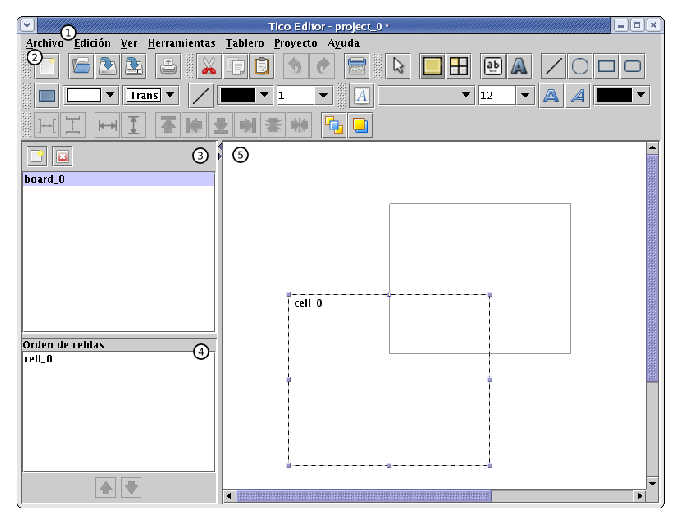
\includegraphics[width=\textwidth]{figures/editor-example}
\caption{Ventana del editor}\label{gra:editor-example}
\end{center}\end{figure}

\par La figura~\ref{gra:editor-example} muestra el aspecto de la ventana principal del
Editor. En ella se pueden distinguir los siguientes elementos:
\begin{enumerate}
	\item \textbf{Barra de men�:} Permite realizar la mayor�a de las acciones aplicables a un tablero.
	\item \textbf{Barras de herramientas:} Conjunto de barras de herramientas m�viles dirigidas a la edici�n de tableros y las propiedades de sus componentes.
	\item \textbf{Lista de tableros del proyecto:} Lista con los tableros pertenecientes al proyecto actual. Permite seleccionar cu�l es el tablero que se quiere editar en cada momento.
	\item \textbf{Orden de barrido del proyecto seleccionado:} Muestra y permite editar el orden de barrido de las celdas mostradas en un determinado momento.
	\item \textbf{�rea de edici�n:} Elemento del Editor a trav�s del cual se pueden editar los tableros y sus componentes.
\end{enumerate}

\subsubsection{Barra de men�}
\label{sec:manual.Editor.elementos.menu}

\par La barra de men� de la aplicaci�n contiene los siguientes submen�s
que permiten realizar todo tipo de acciones sobre el Editor. Las acciones
concretas se mostrar�n en los lugares correspondientes seg�n la funci�n que
realicen. Los submen�s son los siguientes:
\begin{itemize}
	\item \textbf{Archivo}: Acciones a realizar sobre un proyecto. Permite crear
	un proyecto nuevo tanto normal como para Android, cargarlo, guardarlo, exportarlo a diferentes formatos, importarlo, imprimirlo y salir de la aplicaci�n.
	\item \textbf{Edici�n}: Acciones b�sicas de edici�n. Permite deshacer y rehacer, cortar copiar y pegar componentes,	borrar los componentes seleccionados, seleccionar todo y editar las preferencias de la aplicaci�n.
	\item \textbf{Ver}: Permite mostrar y ocultar las barras de herramientas de la aplicaci�n.
	\item \textbf{Herramientas}: Especifica la herramienta de edici�n actual, una por cada
	componente que se puede insertar en un tablero y otra para seleccionar componentes, moverlos y redimensionarlos.
	\item \textbf{Tablero}: Contiene las acciones a realizar sobre un tablero.
	\item \textbf{Proyecto}: Contiene las acciones a realizar sobre un proyecto.
	\item \textbf{Ayuda}: Contiene el indispensable ''Acerca de...'' que muestra informaci�n sobre
	la aplicaci�n.
\end{itemize}

\subsubsection{Barras de herramientas}
\label{sec:manual.Editor.elementos.herramientas}

\begin{figure}[h!tb]\begin{center}
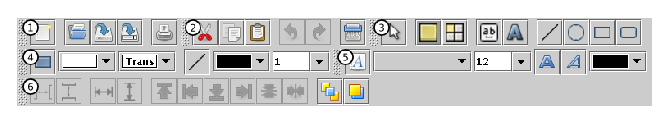
\includegraphics[width=\textwidth]{figures/toolbars}
\caption{Barras de herramientas}\label{gra:toolbars}
\end{center}\end{figure}

\par La ventana del Editor contiene una serie de barras de herramientas independientes
para realizar diferentes tipos de acciones sobre el proyecto que se est� editando.
Estas barras se muestran en la figura~\ref{gra:toolbars} y su funci�n es:
\begin{enumerate}
	\item \textbf{Archivo}: Acciones que se pueden realizar sobre un proyecto.
	\begin{trivlist}
		\item 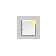
\includegraphics[height=14pt]{figures/toolbar-file-new}
		\textbf{Nuevo proyecto}: Crea un nuevo proyecto.
		\item 
\includegraphics[height=14pt]{figures/archive-new-android-22}
		\textbf{Nuevo proyecto Android}: Crea un nuevo proyecto para Android.		
		\item 
\includegraphics[height=14pt]{figures/toolbar-file-open}
		\textbf{Abrir proyecto}: Carga un proyecto desde un fichero de proyecto. Se puede cambiar el filtro de archivos entre proyectos normales y proyectos para Android.
		\item 
\includegraphics[height=14pt]{figures/toolbar-file-save}
		\textbf{Guardar proyecto}: Graba el proyecto en un fichero con el nombre
		actual o pregunta el nombre y el tipo si a�n no ha sido especificado.
		\item 
\includegraphics[height=14pt]{figures/toolbar-file-save-as}
		\textbf{Guardar proyecto como}: Graba el proyecto en un fichero preguntando
		el nombre del mismo. Se puede cambiar tambi�n el tipo de proyecto, si es un proyecto para su interpetaci�n en el Int�rprete normal o para el Int�rprete Android.
		\item 
\includegraphics[height=14pt]{figures/toolbar-file-print}
		\textbf{Imprimir proyecto}: Imprime el proyecto de forma que cada tablero
		queda en una p�gina diferente.
	\end{trivlist}
	\item \textbf{Acciones}: Acciones que se pueden realizar sobre el tablero en edici�n.
	\begin{trivlist}
		\item 
\includegraphics[height=14pt]{figures/toolbar-edit-cut}
		\textbf{Cortar}: Corta los elementos del �rea de edici�n que est�n seleccionados
		en el portapapeles.
		\item 
\includegraphics[height=14pt]{figures/toolbar-edit-copy}
		\textbf{Copiar}: Copia los elementos del �rea de edici�n que est�n seleccionados
		en el portapapeles.
		\item 
\includegraphics[height=14pt]{figures/toolbar-edit-paste}
		\textbf{Pegar}: Pega en el tablero que se est� editando el contenido del portapapeles.
		\item 
\includegraphics[height=14pt]{figures/toolbar-edit-undo}
		\textbf{Deshacer}: Deshace la �ltima modificaci�n realizada en tablero en edici�n.
		\item 
\includegraphics[height=14pt]{figures/toolbar-edit-redo}
		\textbf{Rehacer}: Rehace la �ltima modificaci�n deshecha en tablero en edici�n.
		\item 
\includegraphics[height=14pt]{figures/toolbar-edit-delete}
		\textbf{Borrar}: Borra los elementos seleccionados en el �rea de edici�n.
	\end{trivlist}
	\item \textbf{Herramientas}: Selecciona la herramienta que se va a utilizar para interaccionar con el �rea de edici�n. Las herramientas se utilizan pulsando con el rat�n sobre el �rea de edici�n	y arrastrando hasta conseguir el tama�o deseado. Cuando se haya insertado un componente la herramienta	activada cambiar� autom�ticamente a la de selecci�n. El bot�n que corresponde con la herramienta	seleccionada en el momento actual est� siempre resaltado.
	\begin{trivlist}
		\item 
\includegraphics[height=14pt]{figures/toolbar-actions-select}
		\textbf{Selecci�n}: Permite seleccionar, redimensionar y mover componentes o conjuntos
		de ellos. Realizando \textit{doble-clic} sobre cualquier componente se muestran
		sus propiedades y pulsando con el bot�n derecho ofrece una serie de acciones a realizar
		relacionadas con el componente.
		\item 
\includegraphics[height=14pt]{figures/toolbar-actions-cell}
		\textbf{Celda}: Herramienta para crear celdas.
		\item 
\includegraphics[height=14pt]{figures/handler-cell-controller-22}
		\textbf{Celda de control}: Herramienta para celdas de control.
		\item 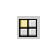
\includegraphics[height=14pt]{figures/toolbar-actions-grid}
		\textbf{Cuadr�cula}: Herramienta para crear cuadr�culas. Al seleccionarla te abre un di�logo que te pregunta la dimensi�n de la cuadr�cula que quieres crear.
		\item 
\includegraphics[height=14pt]{figures/toolbar-actions-text-area}
		\textbf{�rea de texto}: Herramienta para crear �reas de texto.
		\item 
\includegraphics[height=14pt]{figures/toolbar-actions-label}
		\textbf{Etiqueta}: Herramienta para crear etiquetas.
		\item 
\includegraphics[height=14pt]{figures/toolbar-actions-line}
		\textbf{L�nea}: Herramienta para crear l�neas.
		\item 
\includegraphics[height=14pt]{figures/toolbar-actions-oval}
		\textbf{�valo}: Herramienta para crear �valos.
		\item 
\includegraphics[height=14pt]{figures/toolbar-actions-rectangle}
		\textbf{Rect�ngulo}: Herramienta para crear rect�ngulos.
		\item 
\includegraphics[height=14pt]{figures/toolbar-actions-round-rect}
		\textbf{Rect�ngulo redondeado}: Herramienta para crear rect�ngulos redondeados.
	\end{trivlist}
	\item \textbf{Formato}: Determina las propiedades del fondo y borde que tendr�n los nuevos componentes. Cuando se selecciona alg�n componente en el �rea de edici�n, esta barra de herramientas se actualiza autom�ticamente para reflejar las propiedades de fondo y borde de ese componente. Si se quieren	cambiar las propiedades del fondo y borde de todos los componentes seleccionados en el �rea de edici�n	hay que modificar los par�metros correspondientes y pulsar sobre el bot�n que corresponda a las	propiedades que se quieren modificar.
	\begin{trivlist}
		\item 
\includegraphics[height=14pt]{figures/toolbar-format-apply-background}
		\textbf{Aplicar fondo}: Modifica las propiedades del fondo de los componentes seleccionados
		a los elegidos en el resto de elementos de la barra de herramientas a la que pertenece.
		\item 
\includegraphics[height=14pt]{figures/toolbar-format-apply-border}
		\textbf{Aplicar borde}: Modifica las propiedades del borde de los componentes seleccionados
		a los elegidos en el resto de elementos de la barra de herramientas a la que pertenece.
	\end{trivlist}
	\item \textbf{Texto}: Determina la fuente de texto que tendr�n todos los nuevos componentes. Cuando se selecciona alg�n componente en el �rea de edici�n, esta barra de herramientas se actualiza autom�ticamente para reflejar la fuente de ese componente. Si se quiere cambiar la fuente de todos los componentes seleccionados en el �rea de edici�n, hay que modificar los par�metros correspondientes y pulsar sobre el bot�n \textit{Aplicar fuente}.
	\begin{trivlist}
		\item 
\includegraphics[height=14pt]{figures/toolbar-text-apply-font}
		\textbf{Aplicar fuente}: Modifica las fuente de los componentes seleccionados a los elegidos en el resto de elementos de la barra de herramientas a la que pertenece.
	\end{trivlist}
	
	\item \textbf{Alineaci�n}: Opciones de alineaci�n entre grupos de componentes seleccionados
de un tablero.

	\begin{trivlist}
		\item 
\includegraphics[height=14pt]{figures/toolbar-align-horizontal-gap}
		\textbf{Separaci�n horizontal}: Distribuye los componentes seleccionados horizontalmente de forma que los de los extremos se queden en su sitio y el resto se distribuyan para que el espacio que los separe sea id�ntico para todos ellos.
		\item 
\includegraphics[height=14pt]{figures/toolbar-align-vertical-gap}
		\textbf{Separaci�n vertical}: Distribuye los componentes seleccionados verticalmente de forma que los de los extremos se queden en su sitio y el resto se distribuyan para que el espacio que los separe sea id�ntico para todos ellos.
		\item 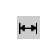
\includegraphics[height=14pt]{figures/toolbar-align-adjust-width}
		\textbf{Ajustar anchura}: Asigna a todos los elementos seleccionados la anchura del primero que	se seleccion�.
		\item 
\includegraphics[height=14pt]{figures/toolbar-align-adjust-height}
		\textbf{Ajustar altura}: Asigna a todo los elementos seleccionados la altura del primero que se seleccion�.
		\item 
\includegraphics[height=14pt]{figures/toolbar-align-top}
		\textbf{Alinear arriba}: Alinea todos los elementos seleccionados de forma que sus lados superiores queden en l�nea con el del primero que se seleccion�.
		\item 
\includegraphics[height=14pt]{figures/toolbar-align-left}
		\textbf{Alinear izquierda} Alinea todos los elementos seleccionados de forma que sus lados izquierdos queden en l�nea con el del primero que se seleccion�.
		\item 
\includegraphics[height=14pt]{figures/toolbar-align-bottom}
		\textbf{Alinear abajo}: Alinea todos los elementos seleccionados de forma que sus lados inferiores queden en l�nea con el del primero que se seleccion�.
		\item 
\includegraphics[height=14pt]{figures/toolbar-align-right}
		\textbf{Alinear derecha}: Alinea todos los elementos seleccionados de forma que sus lados derechos queden en l�nea con el del  primero que se seleccion�.
		\item 
\includegraphics[height=14pt]{figures/toolbar-align-horizontal-center}
		\textbf{Alinear centro horizontal}: Alinea todos los elementos seleccionados de forma que sus ejes horizontales queden en l��nea con el del primero que se seleccion�.
		\item 
\includegraphics[height=14pt]{figures/toolbar-align-vertical-center}
		\textbf{Alinear centro vertical}: Alinea todos los elementos seleccionados de forma que sus ejes verticales queden en l��nea con el del primero que se seleccion�.
		\item 
\includegraphics[height=14pt]{figures/toolbar-align-front}
		\textbf{Enviar al frente}: Env�a al frente todos los objetos seleccionados de forma que se muestran por encima de los dem�s.
		\item 
\includegraphics[height=14pt]{figures/toolbar-align-back}
		\textbf{Enviar al fondo}: Env�a al fondo todos los objetos seleccionados de forma que se muestran debajo de los dem�s.
	\end{trivlist}
\end{enumerate}
\par Todas ellas pueden ser mostradas u ocultadas a trav�s del men� \textit{Ver}
de la aplicaci�n. Por defecto se sit�an en la parte superior de la ventana del Editor,
pero pueden ser desplazadas a cualquier punto de la pantalla pulsando y arrastrando en
la parte punteada situada a la izquierda de cada una de ellas.

\par Si las acciones que corresponden a cada uno de los elementos de una barra de herramientas
no se pueden realizar, ser�n deshabilitadas y los botones que las invocan se mostrar�n en blanco y negro.

\subsubsection{Preferencias del Editor}
\label{sec:manual.Editor.elementos.preferencias}

\par Las preferencias del Editor se pueden modificar pulsando \textit{Editar - Preferencias}.
Las preferencias son:
\begin{itemize}
	\item \textbf{Idioma:} Especifica el idioma de ejecuci�n de la aplicaci�n. Para cambiarlo
	hay que reiniciar la aplicaci�n.
\end{itemize}

% Edición de proyectos
\subsection{Edici�n de proyectos}\label{sec:manual.Editor.proyectos}

\par La aplicaci�n del Editor est� dise�ada para editar proyectos, tanto para su interpretaci�n en un ordenador personal como en un dispositivo Android, y los tableros que la componen. Para a�adir y borrar tableros a un proyecto se utiliza la \textit{lista de tableros}, la cual tambi�n permite seleccionar qu� tablero se va a mostrar en el �rea de edici�n.

\subsubsection{Acciones sobre un proyecto}
\label{sec:manual.Editor.proyecto.acciones}

\par A trav�s de la barra de men� y en algunos casos de su correspondiente bot�n en la barra de herramientas, se pueden realizar las siguientes acciones sobre el proyecto actual:
\begin{itemize}
	\item \textbf{Guardar:} Guarda el proyecto en un fichero para que pueda ser abierto, ya sea para ser interpretado o seguir siendo editado posteriormente. Se puede seleccionar el tipo de proyecto que es, entre \textit{proyectos de Tico} para su interpretaci�n en un ordenador personal y \textit{proyectos de Tico Android} para su interpretaci�n en un dispositivo Android.
	\item \textbf{Imprimir:} Imprime el proyecto entero de forma que cada tablero se imprima	en una hoja diferente.
	\item \textbf{Importar un proyecto:} Importa un proyecto guardado previamente y a�ade todos sus tableros a la lista de tableros del proyecto manteniendo las relaciones de navegaci�n entre ellos.
	\item \textbf{Importar un tablero:} Importa un tablero exportado previamente y lo a�ade a la lista de tableros del proyecto.
	\item \textbf{Exportar el tablero seleccionado:} Exporta el tablero seleccionado a un fichero \textit{.brd} para que pueda ser importado y reutilizado posteriormente en otro proyecto.
	\item \textbf{Exportar el tablero seleccionado a una imagen:} Exporta el tablero seleccionado a un fichero de imagen en formato \textsl{JPG} o \textsl{PNG}.
	\item \textbf{Modificar sus propiedades:} Las propiedades de un proyecto se pueden modificar a trav�s de una ventana que se abre ejecutando \textit{Proyecto - Propiedades}.
\end{itemize}

\subsubsection{Lista de tableros}
\label{sec:manual.Editor.proyectos.tableros}

\begin{figure}[h!tb]\begin{center}
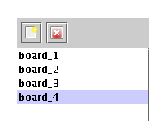
\includegraphics[width=0.4\textwidth]{figures/board-list}
\caption{Lista de tableros}\label{gra:board-list}
\end{center}\end{figure}

\par La lista de tableros se muestra en la figura~\ref{gra:board-list}. Tiene dos botones que permiten a�adir y borrar tableros del proyecto y una lista en la cual se seleccionar el tablero que se quiere editar en cada momento. El bot�n 
\includegraphics[height=11pt]{figures/board-list-new} a�ade un nuevo tablero vac�o al proyecto y el bot�n 
\includegraphics[height=11pt]{figures/board-list-delete} borra el tablero seleccionado. La acci�n de borrar un tablero no se puede deshacer, as� que antes de realizarla habr� que cerciorarse de que el tablero seleccionado no se necesita.

\subsubsection{Propiedades de un proyecto}
\label{sec:manual.Editor.proyectos.propiedades}

\par Las propiedades del proyecto actual se pueden modificar pulsando \textit{Proyecto - Propiedades}. La ventana de propiedades se puede reescalar y si se reduce se podr� tener acceso a todos sus componentes mediante scroll vertical y horizontal. 
\par Estas propiedades son:
\begin{itemize}
	\item \textbf{Tablero inicial:} Determina el primer tablero que se abrir� cuando se inicie la
	interpretaci�n el proyecto.
	\item \textbf{Orientaci�n (s�lo en edici�n para Android):} Determina la orientaci�n de pantalla que se forzar� en el Int�rprete TICO4Android para la visualizaci�n del proyecto. Las opciones son:
	\begin{itemize}
		\item \textbf{Vertical:} El proyecto en el Int�rprete TICO4Android se visualizar� de forma vertical, en la posici�n en que la pantalla es m�s alta que ancha. El proyecto no se reorientar� al cambiar la posici�n del dispositivo Android.
		\item \textbf{Horizontal:} El proyecto en el Int�rprete TICO4Android se visualizar� de forma horizontal, en la posici�n en que la pantalla es m�s ancha que alta. El proyecto no se reorientar� al cambiar la posici�n del dispositivo Android.
		\item \textbf{Libre:} El proyecto en el Int�rprete TICO4Android se visualizar� de la forma en la que est� orientado el dispositivo Android. Durante la ejecuci�n si se reorienta el dispositivo autom�ticamente tambi�n se reorientar� el proyecto.
	\end{itemize}
\end{itemize}

% ��rea de edici�n de tableros
\subsection{Edici�n de tableros} \label{sec:manual.Editor.tablero}

\par Para editar un tablero se proveen una serie de herramientas que permiten al usuario interaccionar con el \textit{�rea de edici�n}. Su funcionamiento se explica en los siguientes apartados.

\subsubsection{�rea de edici�n}
\label{sec:manual.Editor.tablero.area}

\par El �rea de edici�n muestra el tablero seleccionado en la \textit{lista de tableros} del proyecto actual. Para interaccionar con ella hay que elegir la herramienta que se quiere utilizar, ya sea a trav�s del submen� \textit{Herramientas} de la aplicaci�n o de la barra de herramientas del mismo nombre.

\par Las herramientas se pueden dividir en dos grupos:
\begin{itemize}
	\item \textbf{Herramientas que sirven para insertar nuevos componentes en el tablero.} Dentro de este grupo existe una herramienta diferente para cada tipo de componente, pero todas ellas funcionan de manera similar. Una vez seleccionada, se pulsa con el rat�n en un punto del tablero y se arrastra hasta haber obtenido el tama�o deseado.
	\item \textbf{Herramientas para interaccionar con el tablero.} Dentro de este grupo �nicamente est� la herramienta de selecci�n. Las utilidades de esta herramienta son muchas:
	\begin{itemize}
		\item \textbf{Seleccionar componentes:} Permite seleccionar componentes y grupos de ellos. Esto se puede realizar de varias formas. Pulsando con el bot�n izquierdo del rat�n sobre un componente, lo seleccionas y deseleccionas todos los dem�s. Si adem�s est�s pulsando la tecla \textit{control}, a�ades el nuevo componente a la selecci�n actual. Lo mismo se puede realizar pulsando y arrastrando, en este caso se seleccionar�n todos los componentes que se encuentren dentro del cuadrado de selecci�n.
		\item \textbf{Redimensionar componentes:} Los componentes individuales seleccionados
se pueden redimensionar pulsando y arrastrando en cualquiera de las peque�as marcas que aparecen en las esquinas del rect�ngulo de selecci�n y en el centro de cualquiera de sus lados. El icono que aparece al poner el rat�n sobre ellas muestra las direcciones en las que permiten redimensionar.
		\item \textbf{Mover componentes:} Un componente o conjunto de componentes seleccionados se puede desplazar en el tablero pulsando sobre cualquiera de ellos y arrastr�ndolo hasta situarlo en el lugar deseado.
		\item \textbf{Mostrar ventana de propiedades de componentes:} Haciendo \textit{doble-clic} con el rat�n sobre cualquier componente del tablero se abre la ventana que permite editar las propiedades de ese componente.
		\item \textbf{Mostrar men�s desplegables:} Pulsando el bot�n derecho del rat�n sobre cualquier punto del tablero o cualquiera de sus componentes se muestra un men� desplegable que permite realizar diferentes acciones relacionadas con el tablero o con el componente pulsado.
	\end{itemize}
\end{itemize}

\subsubsection{Orden de barrido}
\label{sec:manual.Editor.tablero.barrido}

\par Determina el orden de barrido de las celdas del tablero actual. Cuando una de ellas se a�ade a un tablero tambi�n se a�ade autom�ticamente al final del orden de barrido del mismo. Se puede modificar el orden seleccionando el componente que se quiere mover y pulsando sobre los botones 
\includegraphics[height=11pt]{figures/cell-order-up} o 
\includegraphics[height=11pt]{figures/cell-order-down} para adelantarlo o retrasarlo en el orden respectivamente.

\subsubsection{Propiedades de un tablero}
\label{sec:manual.Editor.tablero.propiedades}

\par Para mostrar la ventana de propiedades del tablero se puede pulsar \textit{Tablero - Propiedades} o, con la herramienta de selecci�n activada, pulsar el bot�n derecho sobre el fondo del tablero en el �rea de edici�n y seleccionar \textit{Propiedades}. La ventana de propiedades se puede reescalar y si se reduce se podr� tener acceso a todos sus componentes mediante scroll vertical y horizontal.

\par Las propiedades de un tablero son:
\begin{itemize}
	\item \textbf{Nombre:} Nombre del tablero que se mostrar� en la lista de tableros.
	\item \textbf{Tama�o:} Tama�o del tablero en \textsl{p�xeles}.
	\item \textbf{Color de fondo:} Color de fondo del tablero. Tambi�n se puede seleccionar un color de gradiente para hacer un degradado en el tablero.
	\item \textbf{Sonido de fondo:} Sonido que se reproducir� al cargar el tablero en el Int�rprete durante la interpretaci�n del mismo.
	\item \textbf{Imagen de fondo:} Imagen de fondo del tablero. Para seleccionar como se ajusta la imagen al tama�o del tablero se ofrecen tres opciones:
	\begin{itemize}
		\item \textbf{Centrada:} La imagen se centra dentro del tablero. Si la imagen es mayor que el tablero se reduce, pero sin perder sus proporciones.
		\item \textbf{Redimensionada:} La imagen se redimensiona para que se ajuste al ancho o al alto del tablero de forma que no pierda sus proporciones.
		\item \textbf{Ajustada:} La imagen se redimensiona de forma que cubra todo el fondo del tablero.
	\end{itemize}
	\item \textbf{Orden de barrido:} Determina el orden de barrido de las celdas del tablero. Esta lista es la misma que se permite editar a trav�s de la ventana principal del Editor. El interfaz que permite modificarlo se muestra en la figura~\ref{gra:board-properties-order-component}. La lista inferior es id�ntica a la mostrada en la ventana principal del Editor. La superior contiene las celdas que no se quiere que sean barridas. Para moverlas de una lista a otra se utilizan los botones 
\includegraphics[height=11pt]{figures/board-properties-order-add} y 
\includegraphics[height=11pt]{figures/board-properties-order-remove} que permiten a�adir a la lista inferior el elemento seleccionado de la superior y viceversa.
\end{itemize}

\begin{figure}[htb]\begin{center}
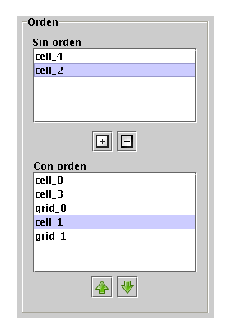
\includegraphics[width=0.4\textwidth]{figures/board-properties-order-component}
\caption{Interfaz de edici�n de orden de barrido}\label{gra:board-properties-order-component}
\end{center}\end{figure}

% Componentes de un tablero
\subsection{Componentes de un tablero}\label{sec:manual.Editor.componentes}

\par En esta secci�n se definen todos los posibles componentes de un tablero y sus propiedades. Como ya se ha explicado en la secci�n~\ref{sec:manual.Editor.tablero}, para insertar un nuevo componente hay que utilizar la herramienta correspondiente al tipo de componente que se quiere insertar. En la figura~\ref{gra:component-examples} se puede ver un ejemplo de cada tipo de componente.

\begin{figure}
\begin{tabular}{ccc}
	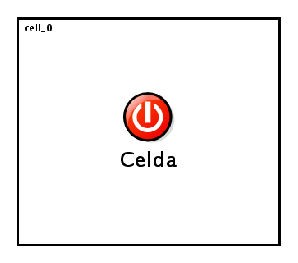
\includegraphics[width=0.3\textwidth]{figures/component-examples-cell} &
	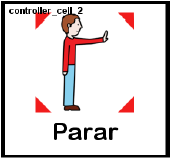
\includegraphics[width=0.3\textwidth]{figures/component-examples-control-cell} &	
	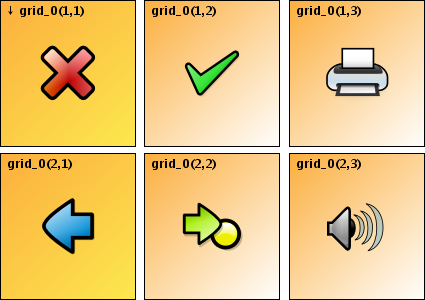
\includegraphics[width=0.3\textwidth]{figures/component-examples-grid} \\
	
	Celda & Celda de control & Cuadr�cula \\ \\
	\includegraphics[width=0.3\textwidth]{figures/component-examples-text-area}	&
	\includegraphics[width=0.3\textwidth]{figures/component-examples-label} &
	\includegraphics[width=0.3\textwidth]{figures/component-examples-line} \\
	�rea de texto & Etiqueta & L�nea \\ \\
	\includegraphics[width=0.3\textwidth]{figures/component-examples-rectangle} &
	\includegraphics[width=0.3\textwidth]{figures/component-examples-round-rect} &
	\includegraphics[width=0.3\textwidth]{figures/component-examples-oval} \\
	Rect�ngulo & Rect�ngulo redondeado & �valo \\ \\
\end{tabular}
\caption{Ejemplos de componentes}\label{gra:component-examples}
\end{figure}

\par Para mostrar la ventana de propiedades de un componente, con la herramienta de selecci�n activada, hay que hacer \textit{doble-clic} o pulsar el bot�n derecho y seleccionar \textit{Propiedades} sobre el componente que se quiere modificar. Las ventanas de propiedades de los distintos elementos son muy similares. Todas ellas est�n formadas por un componente en el que las propiedades est�n agrupadas por solapas, tres botones que permiten aceptar, aplicar o cancelar respectivamente las propiedades elegidas y, en algunos casos, un campo de texto que permite especificar el identificador del componente. La ventana de propiedades se puede reescalar y si se reduce se podr� tener acceso a todos sus componentes mediante scroll vertical y horizontal. La figura~\ref{gra:cell-dialog-examples} muestra un ejemplo de la ventana de propiedades de una celda.

\begin{figure}
\begin{minipage}{0.45\textwidth}\begin{center}
\includegraphics[width=\textwidth]{figures/cell-dialog-examples-1}
\end{center}\end{minipage}
\hfill
\begin{minipage}{0.45\textwidth}\begin{center}
\includegraphics[width=\textwidth]{figures/cell-dialog-examples-2}
\end{center}\end{minipage}
\hfill
\begin{minipage}{0.45\textwidth}\begin{center}
\includegraphics[width=\textwidth]{figures/cell-dialog-examples-3}
\end{center}\end{minipage}
\hfill
\begin{minipage}{0.45\textwidth}\begin{center}
\includegraphics[width=\textwidth]{figures/cell-dialog-examples-4}
\end{center}\end{minipage}
\caption{Ventanas de propiedades de una celda}\label{gra:cell-dialog-examples}
\end{figure}
	
\subsubsection{Celdas}
\label{sec:manual.Editor.componentes.celdas}

\par Las celdas son los componentes principales de un tablero. Junto con las celdas de control son los elementos con los que el usuario puede interaccionar directamente durante la interpretaci�n.

\par Las propiedades de una celda son:
\begin{itemize}
	\item \textbf{Identificador:} Identificador �nico dentro de su tablero que determina la celda y que se muestra en todos los interfaces donde �sta puede ser seleccionada.
	\item \textbf{Texto:} Texto que se muestra centrado verticalmente.
	\item \textbf{Fuente:} Fuente que se le aplica al texto de la celda. En la edici�n Android no se puede seleccionar ya que se usa la fuente de Android.
	\item \textbf{Borde:} Anchura y color del borde rectangular que rodea la celda.
	\item \textbf{Efectos de barrido:} Anchura y color del borde rectangular que rodea la celda en el momento del barrido en el Int�rprete.
	\item \textbf{Fondo:} Color del fondo de la celda. Tambi�n se puede seleccionar un color de gradiente para hacer un degradado en el fondo de la celda.
	\item \textbf{Imagen:} Imagen que se mostrar� dentro de la celda. Puede seleccionarse una
imagen existente en el ordenador o bien desde la Galer�a de pictogramas (ver secci�n~\ref{sec:manual.Editor.galeria}). Si la celda tambi�n tiene texto se ofrecen tres opciones de posicionamiento de ambos:
	\begin{itemize}
		\item \textbf{Imagen arriba:} La imagen se sit�a encima del texto dejando un margen entre ambos.
		\item \textbf{Imagen abajo:} La imagen se sit�a debajo del texto dejando un margen entre ambos.
		\item \textbf{Texto centrado:} Ambos elementos se centran en la celda superponi�ndose el texto encima de la imagen.
	\end{itemize}
	\par Aunque en la edici�n Android podemos seleccionar la posici�n del texto, el Int�rprete TICO4Android la ignorar�, ya que la posici�n del texto en este Int�rprete depende de su propia configuraci�n (arriba, abajo o sin texto)
	\item \textbf{Acciones de interpretaci�n:} Estas propiedades determinan las acciones din�micas que realiza la celda durante la interpretaci�n:
	\begin{itemize}
		\item \textbf{Acumular:} Cuando la celda es pulsada se a�ade a una lista que se muestra en la ventana del Int�rprete (ver secci�n~\ref{sec:manual.interprete}). Esta opci�n permite la construcci�n de frases.
		\item \textbf{Ir a otro tablero:} Cuando la celda es pulsada se termina la interpretaci�n del tablero actual y se comienza la del tablero seleccionado. Ambos tableros deber�n pertenecer al mismo proyecto.
		\item \textbf{Imagen alternativa:} Imagen que se muestra cuando el barrido est� sobre la celda o pasamos el rat�n sobre ella.
		\item \textbf{Sonido:} Sonido que se reproduce cuando se pulsa la celda.
		\item \textbf{Texto a enviar:} Cuando la celda es pulsada el texto que contiene se env�a al �rea de texto seleccionada durante el tiempo especificado. Este texto se mostrar� en el �rea en vez del suyo propio original. 
		\item \textbf{V�deo:} V�deo que se reproduce cuando se pulsa la celda.
		\item \textbf{Sonido de barrido:} Sonido que se reproduce cuando el barrido est� sobre la celda. S�lo se reproduce en los modos de barrido y no sonar� si estamos en selecci�n directa. En el Int�rprete Android adem�s tendr� que estar activado en sus opciones el sonido alternativo.
	\end{itemize}
	\item \textbf{Entorno:} Esta propiedad determina la acci�n de control de entorno que debe realizarse al pulsar la celda durante la interpretaci�n.
\end{itemize}


\subsubsection{Celdas de control}
\label{sec:manual.Editor.componentes.celdasDeControl}

\begin{figure}[htb]
\begin{minipage}{0.45\textwidth}\begin{center}
\includegraphics[width=\textwidth]{figures/propiedades-celda-control-1}
\end{center}\end{minipage}
\hfill
\begin{minipage}{0.45\textwidth}\begin{center}
\includegraphics[width=\textwidth]{figures/propiedades-celda-control-2}
\end{center}\end{minipage}

\caption{Ventanas de propiedades de una celda de control}\label{gra:control-cell-dialog-examples}
\end{figure}

\par Las celdas de control son un tipo espec�fico de celdas. Junto con las celdas son los elementos con los que el usuario puede interaccionar directamente durante la interpretaci�n
y permiten controlar las acciones a realizar en el Int�rprete. La figura~\ref{gra:control-cell-dialog-examples} muestra la ventana a trav�s de la que se configura una celda de control.
Las propiedades de una celda de control son:
\begin{itemize}

\item \textbf{Identificador:} Identificador �nico que determina la celda de control y que se
muestra en todos los interfaces donde �sta puede ser seleccionada.
\item \textbf{Texto:} Texto que se muestra en la parte inferior de la celda de control. Este texto no se puede modificar y se corresponde con la acci�n de la celda de control.
\item \textbf{Fuente:} Fuente que se aplica al texto de la celda de control. En la edici�n Android no se puede seleccionar ya que se usa la fuente de Android.
\item \textbf{Acci�n:} Acci�n que realiza la celda de control cuando es pulsada durante la interpretaci�n de un proyecto. Las acciones que se pueden realizar son:
\begin{itemize}
\item \textbf{Leer:} Realiza una lectura de las celdas acumuladas en el �rea de acumulaci�n
del Int�rprete TICO (ver secci�n~\ref{sec:manual.interprete}). La lectura consiste en reproducir por orden el sonido de las celdas acumuladas si lo tienen.
\item \textbf{Volver:} Vuelve al tablero que se interpret� de forma inmediatamente anterior
al tablero actual.
\item \textbf{Inicio:} Vuelve al tablero inicial del proyecto que se est� interpretando.
\item \textbf{Borrar celda:} Borra la �ltima celda acumulada en el �rea de acumulaci�n.
\item \textbf{Borrar celdas:} Borra todas las celdas acumuladas en el �rea de acumulaci�n.
\item \textbf{Parar:} Termina la interpretaci�n del proyecto actual.
\item \textbf {Salir:} Cierra el Int�rprete TICO.
\end{itemize}
\item \textbf{Sonido de barrido:} Sonido que se reproduce cuando el barrido est� sobre la celda. S�lo se reproduce en los modos de barrido y no sonar� si estamos en selecci�n directa. En el Int�rprete TICO4Android adem�s tendr� que estar activado en sus opciones el sonido alternativo.
\end{itemize}

\subsubsection{Cuadr�culas}
\label{sec:manual.Editor.componentes.cuadriculas}

\par Las cuadr�culas son herramientas para crear tablas de celdas de forma r�pida. Pueden ser editadas en conjunto como cuadr�cula despu�s de insertarla mientras estemos editando, pero al ser cargado un proyecto no se recuperar� esa informaci�n y aparecer�n como celdas independientes, sin las opciones de agrupaci�n. Las cuadr�culas no tienen propiedades.


\subsubsection{�reas de texto}
\label{sec:manual.Editor.componentes.areas}

\par Las �reas de texto son componentes rectangulares que pueden contener varias l�neas de texto con diferentes alineaciones. Durante la interpretaci�n de un tablero pueden recibir un texto temporal que se mostrar� durante un tiempo determinado.

\par Las propiedades de una �rea de texto son:
\begin{itemize}
	\item \textbf{Identificador:} Identificador �nico dentro de su tablero que determina el �rea de texto y que se muestra en todos los interfaces donde �sta puede ser seleccionada.
	\item \textbf{Texto:} Texto que se muestra en el �rea de texto.
	\item \textbf{Alineaci�n:} Determina la alineaci�n vertical y horizontal del texto.
	\item \textbf{Fuente:} Fuente que se le aplica al texto. En la edici�n para Android est� deshabilitada ya que se usa la fuente Android.
	\item \textbf{Borde:} Anchura y color del borde rectangular que rodea el �rea de texto.
	\item \textbf{Fondo:} Color del fondo del �rea de texto. Tambi�n se puede seleccionar un color de gradiente para hacer un degradado en el fondo del �rea de texto.
\end{itemize}

\subsubsection{Etiquetas}
\label{sec:manual.Editor.componentes.etiquetas}

\par Las etiquetas son componentes de texto cuyo tama�o se ajusta autom�ticamente.

\par Las propiedades de una etiqueta son:
\begin{itemize}
	\item \textbf{Texto:} Texto que se muestra en la etiqueta.
	\item \textbf{Fuente:} Fuente que se le aplica al texto de la etiqueta. En la edici�n para Android est� deshabilitada ya que se usa la fuente Android.
	\item \textbf{Borde:} Anchura y color del borde rectangular que rodea la etiqueta.
	\item \textbf{Fondo:} Color del fondo de la etiqueta. Tambi�n se puede seleccionar un color de gradiente para hacer un degradado en el fondo de la etiqueta.
\end{itemize}

\subsubsection{L�neas}
\label{sec:manual.Editor.componentes.lineas}

\par Las l�neas son componentes visuales cuya representaci�n es una l�nea que une
dos de las esquinas del componente.

\par Las propiedades de una l�nea son:
\begin{itemize}
	\item \textbf{Color:} Color de dibujo de la l�nea.
	\item \textbf{Anchura:} Anchura de la l�nea.
\end{itemize}

\subsubsection{Pol�gonos}
\label{sec:manual.Editor.componentes.poligonos}

\par Dentro de este grupo se incluyen todos los componentes visuales que tienen id�nticas
propiedades y que �nicamente var�a su forma de representaci�n. Los posibles pol�gonos son:
rect�ngulo, rect�ngulo redondeado y �valo, teniendo cada uno la forma que su nombre indica.

\par Las propiedades de un pol�gono son:
\begin{itemize}
	\item \textbf{Borde:} Anchura y color del borde que rodea el pol�gono.
	\item \textbf{Fondo:} Color del fondo del pol�gono. Tambi�n se puede seleccionar un color de gradiente para hacer un degradado en el fondo del pol�gono.
\end{itemize}

%validacion
\subsection{Utilidad de Validaci�n}\label{sec:manual.Editor.validacion}

\begin{figure}[h!tb]\begin{center}
\includegraphics[width=\textwidth]{figures/utilidades}
\caption{Men� Validaci�n en el Editor}\label{gra:utilidades}
\end{center}\end{figure}

\par Esta opci�n del men� valida tableros y proyectos y administra los elementos relacionados con la validaci�n. La figura~\ref{gra:utilidades} muestra la integraci�n de la herramienta en el Editor.
\par Dentro de esta opci�n se encuentran las distintas alternativas a las que se puede
acceder para manejar la informaci�n que proporciona esta herramienta:

\begin{figure}[h!tb]\begin{center}
\includegraphics[width=\textwidth]{figures/administrar}
\caption{Men� de administraci�n}\label{gra:administrar}
\end{center}\end{figure}

\begin{itemize}
\item \textbf{Administrar:} Facilita el acceso al m�dulo de administraci�n para la edici�n de
los distintos elementos de que est� compuesto (figura~\ref{gra:administrar}).



\begin{itemize}
\item \textbf{Usuarios:} A�ade, modifica o borra usuarios.
\item \textbf{Limitaciones:} Crea o borra limitaciones y permite editar los atributos propios
dentro de cada una de ellas.
\item \textbf{Reglas:} Crea, modifica y borra reglas de validaci�n para posteriores validaciones.
\end{itemize}

\begin{figure}[h!tb]\begin{center}
\includegraphics[width=\textwidth]{figures/validar}
\caption{Men� de validaci�n}\label{gra:validar}
\end{center}\end{figure}

\item \textbf{Validar:} Esta opci�n da paso a la validaci�n completa de tableros y proyectos
(figura~\ref{gra:validar}).
\begin{itemize}
\item \textbf{Tablero:} Hace una validaci�n de los elementos que componen el tablero.
\item \textbf{Proyecto:} Valida el conjunto de tableros de los que est� formado el proyecto y cada tablero por separado.
\end{itemize}


\end{itemize}


\subsubsection{Administraci�n de usuarios}
\label{sec:manual.Editor.validacion.usuarios}

\par La opci�n de administrar usuarios permite al usuario intermedio introducir, modificar o borrar alumnos junto con sus caracter�sticas. Accediendo a trav�s del men� \textit{Utilidades - Validaci�n - Administrar - Usuarios} se alcanzan las opciones de la ventana de la figura~\ref{gra:administracion-usuarios}:

\begin{figure}[h!tb]\begin{center}
\includegraphics[scale=0.75]{figures/administracion-usuarios}
\caption{Ventana para la administraci�n de usuarios}\label{gra:administracion-usuarios}
\end{center}\end{figure}

\begin{itemize}
\item \textbf{Guardar usuario:} Esta opci�n permite:
\begin{itemize}
\item \textbf{A�adir:} Se a�ade un nuevo alumno dando valores a las distintas limitaciones que se muestran en pantalla dentro del rango permitido, escribiendo su nombre en el cuadro editable de la derecha y pulsando el bot�n Guardar usuario.
\item \textbf{Modificar:} Se modifica un alumno que ya se encuentra en la base de datos. Para esto hay que dar valores a las distintas limitaciones dentro del rango permitido, eligiendo en la lista desplegable de la derecha un nombre de entre los que se muestran y pulsando el bot�n Guardar usuario. Como resultado se mostrar� un mensaje informativo si se ha guardado correctamente (figura~\ref{gra:usuario-guardado}) o un mensaje de error en caso contrario.

\begin{figure}[h!tb]\begin{center}
\includegraphics[scale=0.75]{figures/usuario-guardado}
\caption{Usuario guardado}\label{gra:usuario-guardado}
\end{center}\end{figure}

\end{itemize}

\item \textbf{Cargar usuario:} En este caso se cargan los datos de un alumno. Los valores de las limitaciones que aparecen en pantalla se actualizar�n con los que posee el alumno elegido de la lista desplegable de la parte izquierda al pulsar este bot�n (figura~\ref{gra:cargar-usuario}). Esto permite ver las caracter�sticas de un usuario concreto y, si lo creemos conveniente, modificarlo en base a los valores que ya pose�a tal y como se ha explicado anteriormente.
\begin{figure}[h!tb]\begin{center}
\includegraphics[scale=0.75]{figures/cargar-usuario}
\caption{Cargar un usuario}\label{gra:cargar-usuario}
\end{center}\end{figure}


\item \textbf{Borrar usuario:} Eligiendo un alumno de la lista desplegable izquierda y pulsando
el bot�n se le puede eliminar definitivamente. Antes de eliminarlo el sistema muestra un mensaje de confirmaci�n como el de la figura~\ref{gra:borrar-usuario}.
\begin{figure}[h!tb]\begin{center}
\includegraphics[scale=0.75]{figures/borrar-usuario}
\caption{Mensaje de confirmaci�n al borrar un usuario}\label{gra:borrar-usuario}
\end{center}\end{figure}


\end{itemize}

\subsubsection{Administraci�n de limitaciones}
\label{sec:manual.Editor.validacion.administracion-limitaciones}

\par Esta ventana, mostrada en la figura~\ref{gra:administracion-limitaciones}, permite al usuario visualizar y modificar las limitaciones y sus propiedades. Est� compuesta de distintas listas con los nombres de cada limitaci�n y una tabla con los valores dentro de �stas.

\begin{figure}[h!tb]\begin{center}
\includegraphics[width=\textwidth]{figures/administracion-limitaciones}
\caption{Ventana de administraci�n de limitaciones}\label{gra:administracion-limitaciones}
\end{center}\end{figure}

\par Esta ventana permite:

\par En la secci�n \textit{Limitaciones}.
\begin{itemize}
\item \textbf{A�adir limitaci�n:} La nueva limitaci�n queda almacenada escribiendo su nombre en el cuadro editable y pulsando el bot�n.
\item \textbf{Borrar limitaci�n:} Permite borrar una limitaci�n seleccionada de entre las que se encuentran en la lista desplegable al pulsar el bot�n. Inmediatamente aparece un mensaje de confirmaci�n como el de la figura~\ref{gra:borrar-limitacion}.

\begin{figure}[h!tb]\begin{center}
\includegraphics[scale=0.75]{figures/borrar-limitacion}
\caption{Mensaje de confirmaci�n al borrar una limitaci�n}\label{gra:borrar-limitacion}
\end{center}\end{figure}


\end{itemize}

\par En la secci�n \textit{Par�metros}.
\begin{itemize}
\item \textbf{A�adir par�metro:} Se ha de elegir a trav�s de la lista desplegable situada a la izquierda, la limitaci�n en la que se quiere a�adir un par�metro (figura~\ref{gra:cargar-limitacion}); despu�s se escribe en el cuadro editable el nombre del nuevo par�metro y se elige el tipo de dato que va a guardar (num�rico o verdadero/falso); finalmente se pulsa el bot�n.
\begin{figure}%[htb]
\begin{center}
\includegraphics[width=\textwidth]{figures/cargar-limitacion}
\caption{Cargar una limitaci�n}\label{gra:cargar-limitacion}
\end{center}\end{figure}
\item \textbf{Borrar par�metro:} De la misma forma que para a�adir, se elige la limitaci�n, se busca el par�metro de la lista desplegable contigua que se desea borrar y se pulsa el bot�n.

\end{itemize}



\par La secci�n \textit{Requisitos a cumplir} muestra en una tabla los par�metros que contiene cada limitaci�n, cuando en la secci�n \textit{Par�metros} se selecciona alguna de ellas. Tambi�n refleja los cambios que se producen al a�adir o borrar par�metros. La tabla permite modificar el valor de los par�metros y aumentar o disminuir el rango de la limitaci�n.

\begin{itemize}
\item \textbf{A�adir una fila:} En el caso de querer a�adir un nuevo grado al rango de la limitaci�n se ha de pulsar el bot�n \textit{A�adir fila} con lo que, autom�ticamente, aparecer� una nueva fila en la tabla, la cual habr� que rellenar completamente con nuevos datos.

\item \textbf{Borrar una fila completa:} A la hora de disminuir el n�mero de grados de la limitaci�n puede seleccionarse una fila completa, pinchando sobre ella y pulsando el bot�n \textit{Borrar fila completa}.

\item \textbf{Guardar modificaciones:} Una vez modificados los valores de la tabla se pueden guardar pulsando el bot�n. Si se ha a�adido una nueva fila y no se ha completado aparece el mensaje de aviso de la figura~\ref{gra:aviso-fila-incompleta} y el mensaje de error de la figura~\ref{gra:error-guardar-requisitos}.
\begin{figure}%[htb]
\begin{center}
\includegraphics[scale=0.75]{figures/aviso-fila-incompleta}
\caption{Mensaje de aviso para completar todas las filas}\label{gra:aviso-fila-incompleta}
\end{center}\end{figure}

\begin{figure}%[htb]
\begin{center}
\includegraphics[scale=0.75]{figures/error-guardar-requisitos}
\caption{Error al guardar requisitos}\label{gra:error-guardar-requisitos}
\end{center}\end{figure}

\item \textbf{Cargar valores predeterminados:} Los par�metros y los valores que pose�a cada una de las limitaciones que exist�an al inicio de la instalaci�n y que todav�a se encuentran disponibles, son cargados mediante el bot�n Cargar valores predeterminados en la tabla para su visualizaci�n o para ser guardados.

\end{itemize}


\subsubsection{Administraci�n de reglas}
\label{sec:manual.Editor.validacion.administracion-reglas}

\begin{figure}%[htb]
\begin{center}
\includegraphics[width=\textwidth]{figures/administracion-reglas}
\caption{Ventana para la administraci�n de reglas}\label{gra:administracion-reglas}
\end{center}\end{figure}

\par La figura~\ref{gra:administracion-reglas} muestra la ventana que da acceso a la opci�n encargada de administrar las reglas que servir�n para la validaci�n de proyectos. Permite al usuario lo siguiente:


\begin{itemize}
\item \textbf{Modificar regla:} Se puede editar la regla seleccionada mediante la lista desplegable, que puede mostrar todas o s�lo las clasificadas por: reglas para celdas, para tableros o para proyectos mediante los botones de selecci�n. Se muestran sus atributos, par�metros, funci�n utilizada y mensaje a mostrar en sus correspondientes posiciones. Adem�s, para cada una de estas propiedades de la regla se da la opci�n de cambiar cada una de ellas y guardar la regla modificada pulsando el bot�n.

\item \textbf{Borrar regla:} Permite borrar una regla, seleccionando la regla a eliminar de la lista desplegable y pulsando el bot�n.

\item \textbf{A�adir nueva regla:} Se puede insertar una nueva regla pulsando esta opci�n, la cual da paso a una nueva ventana para crear reglas. Como se muestra en la figura~\ref{gra:anyadir-regla} existen listas desplegables para elegir el tipo de funci�n, el/los atributo/s relacionado/s con las caracter�sticas de los componentes del tablero o proyecto que se quieren comprobar, el par�metro con el que se va a hacer la comparaci�n y el mensaje que se quiere mostrar por pantalla. La nueva regla quedar� guardada pulsando el bot�n \textit{Guardar regla} de esta �ltima ventana.

\begin{figure}%[htb]
\begin{center}
\includegraphics[width=\textwidth]{figures/anyadir-regla}
\caption{Ventana para a�adir nuevas reglas}\label{gra:anyadir-regla}
\end{center}\end{figure}

\item \textbf{Cargar reglas predeterminadas:} Se cargar�n autom�ticamente las reglas iniciales (y se borrar�n las a�adidas posteriormente a la instalaci�n de la aplicaci�n) con s�lo pulsar el bot�n, avisando al usuario mediante el mensaje de la figura~\ref{gra:reglas-predeterminadas} si desea continuar con la operaci�n.

\begin{figure}%[htb]
\begin{center}
\includegraphics[width=\textwidth]{figures/reglas-predeterminadas}
\caption{Mensaje de confirmaci�n al cargar las reglas predeterminadas}\label{gra:reglas-predeterminadas}
\end{center}\end{figure}

\end{itemize}

\subsubsection{Validaci�n de tableros}
\label{sec:manual.Editor.validacion.validacion-tableros}

\par La opci�n de validaci�n de tableros, analiza el tablero en s� y todos los componentes dentro de �l. Mediante la figura~\ref{gra:validar-tablero} se muestra el aspecto de la ventana.

\begin{figure}[htb]\begin{center}
\includegraphics[scale=0.75]{figures/validar-tableero}
\caption{Ventana de validaci�n de tableros}\label{gra:validar-tablero}
\end{center}\end{figure}

\par Para comenzar a validar es necesario dar valor a cada limitaci�n o cargar estos valores de alguno de los usuarios que se encuentran en la base de datos, seleccion�ndolos desde la lista desplegable y carg�ndolos mediante el bot�n \textit{Cargar usuario}. Seguidamente se puede validar el tablero mediante el bot�n \textit{Validar}. Se mostrar� una nueva ventana con los resultados del an�lisis, como en la figura~\ref{gra:validacion-tablero}. Tambi�n se puede pedir al sistema un conjunto de sugerencias de dise�o de tableros para poder adaptar nuestro dise�o a los requisitos mostrados. La figura~\ref{gra:sugerencias-tablero} muestra esta �ltima opci�n.

\begin{figure}[h!tb]\begin{center}
\includegraphics[width=\textwidth]{figures/validacion-tablero}
\caption{Ventana de resultados para tableros}\label{gra:validacion-tablero}
\end{center}\end{figure}

\begin{figure}[h!tb]\begin{center}
\includegraphics[width=\textwidth]{figures/sugerencias-tablero}
\caption{Ventana de sugerencias de dise�o para tableros}\label{gra:sugerencias-tablero}
\end{center}\end{figure}

\subsubsection{Validaci�n de proyectos}
\label{sec:manual.Editor.validacion.validacion-proyectos}

\par La validaci�n de proyectos se realiza de la misma manera que la validaci�n de tableros, s�lo que en esta ocasi�n se analiza el proyecto en general y cada uno de los distintos tableros que lo componen en particular. La ventana de validaci�n, que puede verse en la figura~\ref{gra:validar-proyecto}, es muy similar a la de validaci�n de tableros, con las mismas opciones disponibles. Las figuras~\ref{gra:validacion-proyecto} y~\ref{gra:sugerencias-proyecto} muestran los resultados de validar un proyecto y mostrar sugerencias de dise�o respectivamente.

\begin{figure}%[htb]
\begin{center}
\includegraphics[scale=0.75]{figures/validar-proyecto}
\caption{Ventana de validaci�n de proyecto}\label{gra:validar-proyecto}
\end{center}\end{figure}

\begin{figure}%[htb]
\begin{center}
\includegraphics[width=\textwidth]{figures/validacion-proyecto}
\caption{Ventana de resultados para proyectos}\label{gra:validacion-proyecto}
\end{center}\end{figure}

\begin{figure}%[htb]
\begin{center}
\includegraphics[width=\textwidth]{figures/sugerencias-proyecto}
\caption{Ventana de sugerencias de dise�o para proyectos}\label{gra:sugerencias-proyecto}
\end{center}\end{figure}


%galeria de imagenes
\subsection{Utilidad Galer�a de pictogramas}\label{sec:manual.Editor.galeria}
\par Este men� permite la gesti�n de la Galer�a de pictogramas a trav�s de diferentes opciones. La figura~\ref{gra:menu-pictogramas} muestra la integraci�n de esta opci�n en el Editor. \textbf{La Galer�a no va incluida en la instalaci�n de TICO, sino que debe descargarse desde la p�gina web del Proyecto TICO\footnote{\url{http://www.proyectotico.es}} e incorporarse una vez instalado el programa}.
La incorporaci�n de la Galer�a de pictogramas a la aplicaci�n TICO se explica en la secci�n~\ref{sec:manual.Editor.galeria.como-importar} de este manual.

\begin{figure}[h!tb]\begin{center}
\includegraphics[width=\textwidth]{figures/menu-pictogramas}
\caption{Men� Galer�a de pictogramas en el Editor}\label{gra:menu-pictogramas}
\end{center}\end{figure}

\par Los pictogramas incluidos en la Galer�a son elaborados por ARASAAC\footnote{\url{http://www.catedu.es/arasaac}}- CATEDU\footnote{\url{http://www.catedu.es}} con la colaboraci�n de los profesionales del Colegio P�blico de Educaci�n Especial Alborada de Zaragoza y la financiaci�n del Departamento de Ciencia, Tecnolog�a y Universidad del Gobierno de Arag�n y el programa Teruel Digital. Estos pictogramas se distribuyen bajo licencia de Creative Commons (BY-NC-SA).

\par Tambi�n pueden a�adirse im�genes propias a la Galer�a. De esta forma se pueden encontrar r�pidamente para usarlas en los tableros de comunicaci�n generados con TICO.


\subsubsection{C�mo importar la Galer�a de pictogramas en el Editor}
\label{sec:manual.Editor.galeria.como-importar}

\par A continuaci�n se explican los pasos a realizar para importar la Galer�a de pictogramas en el Editor TICO.

\begin{enumerate}
\item Descargar la Galer�a desde la p�gina web de TICO (\url{http://www.proyectotico.es}), que se puede encontrar en la secci�n Galer�a de pictogramas. Guardar el archivo en una ubicaci�n conocida de su equipo, por ejemplo, en el Escritorio.

\item Descomprimir el archivo \textit{Pictogramas.zip} que se habr� descargado. Se generar� la carpeta Pictogramas que debe contener las im�genes.

\item Abrir el Editor TICO. Acceder al men� \textit{Utilidades - Galer�a de pictogramas - Importar Base de Datos}.

\item Pulsar el bot�n \textit{Seleccionar} que abrir� una ventana desde la que podremos seleccionar la carpeta que contiene las im�genes. Deberemos navegar hasta seleccionar la carpeta \textit{Pictogramas}.

\item Si nuestra Galer�a de pictogramas no contiene im�genes antes de importar, pulsamos el bot�n \textit{Importar} y esperamos a que finalice de importar las im�genes.

\item Si ya ten�amos im�genes en la Galer�a y vamos a importarla de nuevo puede ser que haya im�genes que se repitan o tengan el mismo nombre. En este caso podemos elegir entre reemplazar las im�genes que ten�amos por las nuevas, o a�adir las nuevas im�genes a la Galer�a. Una vez seleccionada la opci�n que queremos pulsamos el bot�n \textit{Importar} y esperamos a que finalice de importar las im�genes.

\end{enumerate}

\par Una vez importada la Galer�a se podr�n realizar b�squedas para incorporar im�genes
a los tableros de comunicaci�n.

\subsubsection{B�squeda de im�genes en la Galer�a}
\label{sec:manual.Editor.galeria.busqueda}

\par Dado que el n�mero de pictogramas es muy elevado y sigue en crecimiento, la Galer�a permite la b�squeda de im�genes, tanto por t�rminos clave asociados a las mismas, como por nombre de la imagen. Estos t�rminos clave, que caracterizan una imagen, pueden ser definidos y modificados desde el Editor y son, en principio, los conceptos representados por las im�genes: sin�nimos, traducciones a otros idiomas, etc.

\begin{figure}[h!tb]\begin{center}
\includegraphics[width=\textwidth]{figures/busqueda-imagenes}
\caption{Ventana de b�squeda de im�genes}\label{gra:busqueda-imagenes}
\end{center}\end{figure}

\par La figura~\ref{gra:busqueda-imagenes} muestra la ventana de b�squeda de im�genes. En ella se pueden distinguir los siguientes elementos:

\begin{enumerate}
\item \textbf{Panel de b�squeda por t�rminos clave:} Permite introducir la combinaci�n de t�rminos clave que se quiere buscar y pulsando el bot�n se realiza la b�squeda.

\item \textbf{Panel de b�squeda por nombre:} Permite introducir el nombre de la imagen que se quiere buscar y pulsando el bot�n se realiza la b�squeda.

\item \textbf{Panel de im�genes:} Muestra el resultado de las diferentes b�squedas en grupos de cuatro. Para ver el resto de las im�genes se pueden usar las flechas situadas en la parte inferior o las flechas izquierda y derecha del teclado.
\end{enumerate}

\fbox{ \parbox{0.94 \linewidth}{
\color{red}
	\par Antes de realizar b�squedas es importante saber que:
	
	\begin{itemize}
		\item Cuando se quieren realizar b�squedas de los pictogramas de la Galer�a, �stas deben hacerse por t�rminos clave, no por nombre de la imagen. Esto se debe a que el nombre de la imagen es un c�digo num�rico que la identifica en la Galer�a de pictogramas. De esta forma pueden hacerse b�squedas en los diferentes idiomas disponibles.

		\item La b�squeda por nombre de imagen es �til cuando se han incorporado im�genes externas a la Galer�a.
	
		\item Se puede utilizar el car�cter '*' como comod�n introduciendo tantos asteriscos como se quiera, y en todas las posiciones. La b�squeda por '*' mostrar� como resultado todas las im�genes de la Galer�a.
	\end{itemize}
}}

\begin{itemize}

\item \textbf{B�squeda por t�rminos clave}
\par Permite buscar hasta por tres t�rminos clave.

\par Cuenta con tres cuadros de texto donde se pueden introducir los t�rminos a buscar y dos men�s desplegables donde se puede elegir entre las opciones 'y' y 'o'. Si se elige 'y' se mostrar�n como resultado las im�genes que pertenezcan a todos los t�rminos clave introducidos. Si se elige 'o', se mostrar�n como resultado las im�genes que pertenezcan a alguno de los t�rminos clave introducidos. Estas opciones se pueden combinar para realizar b�squedas m�s complejas.

\par Se puede utilizar el s�mbolo '*' para seleccionar los t�rminos clave que empiezan, acaban o contienen la letra o conjunto de letras introducido. La figura~\ref{gra:ejemplo-busqueda} muestra dos ejemplos de b�squedas en la Galer�a por t�rmino clave.

\begin{figure}
\begin{minipage}{0.95 \textwidth}\begin{center}
\includegraphics[width=\textwidth]{figures/ejemplo-busqueda1}
\end{center}\end{minipage}

\begin{minipage}{0.95 \textwidth}\begin{center}
\includegraphics[width=\textwidth]{figures/ejemplo-busqueda2}
\end{center}\end{minipage}
\caption{Ejemplos de b�squedas de im�genes por t�rmino clave}\label{gra:ejemplo-busqueda}
\end{figure}


\item \textbf{B�squeda por nombre de imagen}

\par Permite buscar im�genes distintas a los pictogramas de ARASAAC que hayan sido insertadas en la Galer�a de la siguiente manera:
\begin{itemize}
\item \textbf{Por nombre exacto de la imagen:} basta con poner el nombre de la imagen que queremos buscar y pulsar en \textit{Buscar}.

\item \textbf{Por nombres que empiecen por una letra o conjunto de letras:} si queremos todos los instrumentos musicales buscaremos por instrumento* y si queremos todas las im�genes que empiecen por la letra 'a' buscaremos a*.

\item \textbf{Por nombres que finalicen por una letra o conjunto de letras:} si queremos todas las palabras que finalicen en 'tor' buscaremos *tor y si queremos todas las palabras que acaban en la letra 'e' buscaremos *e.

\item \textbf{Por nombres que contengan una letra o conjunto de letras:} si queremos todas las palabras que contengan la s�laba 'de' buscaremos *de* y si queremos todas las palabras que contengan una letra 'y' buscaremos por *y*.
\end{itemize}

\par Las figuras~\ref{gra:busqueda-nombre} y~\ref{gra:busqueda-nombre2} muestran dos ejemplos de b�squedas en la Galer�a por nombre de imagen.

\begin{figure}%[htb]
\begin{center}
\includegraphics[width=\textwidth]{figures/busqueda-nombre}
\caption{Ejemplo de b�squeda de imagen por nombre}\label{gra:busqueda-nombre}
\end{center}\end{figure}

\begin{figure}%[htb]
\begin{center}
\includegraphics[width=\textwidth]{figures/busqueda-nombre2}
\caption{Ejemplo de b�squeda de imagen por nombre}\label{gra:busqueda-nombre2}
\end{center}\end{figure}

\end{itemize}

\subsubsection{T�rminos clave}
\label{sec:manual.Editor.galeria.terminos-clave}

\begin{figure}\begin{center}
\includegraphics[scale=0.75]{figures/terminos-clave}
\caption{Ventana para la gesti�n de t�rminos clave}\label{gra:terminos-clave}
\end{center}\end{figure}

\par Esta ventana, mostrada en la figura~\ref{gra:terminos-clave} permite gestionar los t�rminos clave existentes en la Galer�a de pictogramas. Las acciones que se pueden realizar son:

\begin{itemize}
\item \textbf{A�adir:} Se pueden introducir nuevos t�rminos clave escribi�ndolos en el cuadro de texto separados por comas y pulsando despu�s el bot�n \textit{A�adir}.

\item \textbf{Modificar:} Permite modificar un t�rmino clave. Para esto hay que seleccionarlo previamente en la lista lo que provocar� que aparezca escrito en el cuadro de texto. Despu�s de modificarlo en el cuadro de texto pulsamos el bot�n \textit{Modificar}.

\item \textbf{Eliminar:} Permite eliminar el t�rmino clave que se seleccione en la lista. El programa pedir� confirmaci�n de que se desea eliminar el t�rmino.
\end{itemize}

\subsubsection{Insertar imagen}
\label{sec:manual.Editor.galeria.insertar-imagen}

\begin{figure}\begin{center}
\includegraphics[scale=0.75]{figures/insertar-imagen}
\caption{Ventana para insertar una imagen en la Galer�a}\label{gra:insertar-imagen}
\end{center}\end{figure}

\par Esta opci�n permite a�adir una imagen en la Galer�a de pictogramas. La figura~\ref{gra:insertar-imagen} muestra la ventana que permite realizarlo. En ella se pueden distinguir los siguientes elementos:

\begin{enumerate}
\item \textbf{Panel de selecci�n de imagen:} Permite seleccionar la imagen que se desea a�adir a la Galer�a.

\item \textbf{Opciones de inserci�n:} Al a�adir una imagen a la Galer�a puede ser que ya exista otra con el mismo nombre. Este panel permite seleccionar qu� hacer en este caso. Las opciones disponibles son:
\begin{itemize}
\item \textbf{Reemplazar imagen:} Elimina la imagen que hab�a en la Galer�a con sus t�rminos clave y a�ade la nueva imagen con sus t�rminos clave.
\item \textbf{A�adir imagen:} A�ade a la Galer�a la nueva imagen con sus t�rminos clave renombr�ndola. El renombrado de la imagen consiste en a�adir un n�mero al final del nombre de la imagen.
\end{itemize}

\item \textbf{Panel de t�rminos clave:} Permite seleccionar los t�rminos clave que queremos que se asocien con la imagen que vamos a insertar. Adem�s permite a�adir nuevos t�rminos escribi�ndolos en el cuadro de texto separados por comas y pulsando en el bot�n \textit{A�adir}.

\end{enumerate}


\subsubsection{Modificar imagen}
\label{sec:manual.Editor.galeria.modificar}

\par Esta opci�n permite modificar una imagen de la Galer�a de pictogramas. La figura~\ref{gra:modificar-imagen} muestra la ventana que permite realizarlo. A trav�s de ella se pueden realizar b�squedas de im�genes tal y como se explica en la secci�n~\ref{sec:manual.Editor.galeria.busqueda}. Los resultados de las b�squedas se muestran en el panel de im�genes y pinchando sobre ellas se pueden seleccionar para su modificaci�n.

\begin{figure}[h!tb]\begin{center}
\includegraphics[width=\textwidth]{figures/modificar-imagen}
\caption{Ventana para modificar im�genes de la Galer�a}\label{gra:modificar-imagen}
\end{center}\end{figure}

\par Las opciones existentes son:

\begin{enumerate}
\item \textbf{Modificar imagen:} La figura~\ref{gra:modificar} muestra la ventana que se abre al pulsar sobre esta opci�n. A trav�s de ella se pueden modificar los t�rminos clave que est�n asociados a la imagen seleccionando o deseleccionando de la lista de t�rminos. Adem�s se pueden introducir nuevos t�rminos a trav�s del cuadro de texto escribi�ndolos separados por comas y pulsando el bot�n \textit{A�adir}.

\begin{figure}\begin{center}
\includegraphics[scale=0.75]{figures/modificar}
\caption{Ventana para modificar una imagen de la Galer�a}\label{gra:modificar}
\end{center}\end{figure}

\item \textbf{Eliminar imagen:} Pulsando sobre este bot�n se puede eliminar una imagen de la Galer�a. El programa pide confirmaci�n al usuario.
\end{enumerate}

\subsubsection{Eliminar im�genes}
\label{sec:manual.Editor.galeria.eliminar}

\par Esta opci�n permite eliminar varias im�genes de la Galer�a de pictogramas habiendo realizado previamente una b�squeda. La figura~\ref{gra:eliminar-imagen} muestra la ventana que permite realizarlo. A trav�s de ella se pueden realizar b�squedas de im�genes tal y como se explica en la secci�n~\ref{sec:manual.Editor.galeria.busqueda} para ser eliminadas.

\begin{figure}[h!tb]\begin{center}
\includegraphics[width=\textwidth]{figures/eliminar-imagen}
\caption{Ventana para eliminar im�genes de la Galer�a}\label{gra:eliminar-imagen}
\end{center}\end{figure}

\par En esta ventana se distinguen los siguientes elementos:
\begin{enumerate}
\item \textbf{Panel de b�squeda de im�genes:} Este panel permite la b�squeda de im�genes por t�rmino clave o por nombre de imagen para eliminarlas.

\item \textbf{Panel de im�genes:} Este panel permite la visualizaci�n de los resultados de las b�squedas.

\item \textbf{Barra de progreso:} La ventana incorpora una barra de progreso para saber en cada momento la evoluci�n del borrado de im�genes.
\end{enumerate}

\par Las im�genes se eliminan pulsando sobre el bot�n \textit{Eliminar im�genes}.

\subsubsection{Importar Base de Datos}
\label{sec:manual.Editor.galeria.importar}

\par Esta opci�n permite importar una base de datos con el formato adecuado para TICO. Esta base de datos se puede obtener o bien de la p�gina web de TICO (ver secci�n~\ref{sec:manual.Editor.galeria.como-importar}) o exportando la Galer�a de pictogramas del Editor (ver secci�n~\ref{sec:manual.Editor.galeria.exportar}). La figura~\ref{gra:importar} muestra la ventana que permite realizarlo.

\begin{figure}[h!tb]\begin{center}
\includegraphics[width=\textwidth]{figures/importar}
\caption{Ventana para importar la Galer�a de pictogramas}\label{gra:importar}
\end{center}\end{figure}

\par En esta ventana se distinguen los siguientes elementos:
\begin{enumerate}
\item \textbf{Panel de selecci�n de directorio:} Este panel permite la selecci�n del directorio donde se encuentra la base de datos a importar.

\item \textbf{Opciones de importaci�n:} Al importar la base de datos de im�genes en la Galer�a puede ser que ya existan im�genes con el mismo nombre. Este panel permite seleccionar qu� hacer en este caso. Las opciones disponibles son:
\begin{itemize}
\item \textbf{Reemplazar imagen:} Elimina la imagen que hab�a en la Galer�a con sus t�rminos clave y a�ade la nueva imagen con sus t�rminos clave.
\item \textbf{A�adir imagen:} A�ade a la Galer�a la nueva imagen con sus t�rminos clave renombr�ndola. El renombrado de la imagen consiste en a�adir un n�mero al final del nombre de la imagen.
\end{itemize}

\item \textbf{Barra de progreso:} La ventana lleva incorporada una barra de progreso para que el usuario conozca en cada momento el estado de la importaci�n.

\end{enumerate}

\par Pulsando el bot�n \textit{Importar} comienza la importaci�n de la base de datos.

\subsubsection{Exportar Base de Datos}
\label{sec:manual.Editor.galeria.exportar}

\par Esta opci�n permite realizar b�squedas de im�genes tal y como se explica en la secci�n~\ref{sec:manual.Editor.galeria.busqueda}. para exportarlas a una base de datos que podr� ser importada posteriormente. La figura 40 muestra la ventana que permite realizarlo.

\begin{figure}[h!tb]\begin{center}
\includegraphics[width=\textwidth]{figures/exportar}
\caption{Ventana para exportar la Galer�a de pictogramas}\label{gra:exportar}
\end{center}\end{figure}

\par En esta ventana se distinguen los siguientes elementos:
\begin{enumerate}
\item \textbf{Panel de b�squeda de im�genes:} Este panel permite la b�squeda de im�genes por t�rmino clave o por nombre de imagen. Es necesario realizar una b�squeda que indique las im�genes a exportar. En el panel de im�genes se muestran los resultados de las b�squedas.
\item \textbf{Panel de selecci�n de directorio:} Este panel permite la selecci�n del directorio donde se guardar� la Galer�a de pictogramas exportada.
\item \textbf{Barra de progreso:} La ventana lleva incorporada una barra de progreso para
que el usuario conozca en cada momento el estado de la exportaci�n.

\end{enumerate}
\par Pulsando el bot�n \textit{Exportar} comienza la exportaci�n de la base de datos.


\subsection{Modos de edici�n: Normal y Android}
\label{sec:manual.Editor.modos}
\par El Editor TICO puede ser usado para crear proyectos TICO tanto para el Int�rprete normal de ordenador personal, como para el Int�rprete TICO4Android. Los archivos resultantes para proyectos normales y Android tienen las extensiones \textit{.tco} y \textit{.tcoa} respectivamente.

\par El funcionamiento, aspecto y opciones de ambos modos de edici�n son muy similares aunque con algunas diferencias. Durante la edici�n, en todo momento podemos saber en qu� modo estamos editando mirando la barra superior de la aplicaci�n. Si estamos en modo Normal en la barra superior aparecer� escrito \textit{Editor Tico -} y el nombre del proyecto que est� siendo editado (ver figura~\ref{gra:modo-normal}). Si estamos en modo Android aparecer� escrito \textit{Editor Tico ANDROID -} y el nombre del proyecto que est� siendo editado (ver figura~\ref{gra:modo-android}).

\begin{figure}[h!tb]\begin{center}
\includegraphics[width=\textwidth]{figures/modo-normal}
\caption{Barra de la aplicaci�n Editor en modo Normal}\label{gra:modo-normal}
\end{center}\end{figure}

\begin{figure}[h!tb]\begin{center}
\includegraphics[width=\textwidth]{figures/modo-android}
\caption{Barra de la aplicaci�n Editor en modo Android}\label{gra:modo-android}
\end{center}\end{figure}

\par El cambio de un modo a otro es autom�tico y depende de nuestras decisiones al crear un nuevo proyecto, abrir o guardar. El modo de edici�n puede cambiar entre Normal y Android en los siguientes casos:
\begin{itemize}
	\item \textbf{Al crear un nuevo proyecto.} Para crear un nuevo proyecto tenemos dos opciones, tanto en la barra de herramientas como en los iconos, \textit{Nuevo} y \textit{Nuevo android} que crear�n un proyecto nuevo en modo Normal o modo Android respectivamente.
	
	\item \textbf{Al abrir un proyecto existente.} En el di�logo de selecci�n de archivo (ver figura~\ref{gra:abrir-proyecto}) podemos cambiar el filtro en \textit{Archivos de Tipo} entre \textit{Proyectos de Tico} y \textit{Proyectos de Tico Android}. Si terminamos correctamente de abrir un proyecto el Editor estar� en el modo del tipo aqu� seleccionado.


\begin{figure}[htb]\begin{center}
\includegraphics[width=\textwidth]{figures/abrir-proyecto}
\caption{Ventana para la selecci�n de proyecto a abrir}\label{gra:abrir-proyecto}
\end{center}\end{figure}

\item \textbf{Al guardar un proyecto.} De la misma forma que al abrir, en el di�logo de selecci�n de archivo para guardar (el cual aparece al seleccionar \textit{Guardar como} o al seleccionar \textit{Guardar} sin que se haya especificado previamente su nombre) podemos cambiar el tipo de proyecto entre \textit{Proyectos de Tico} y \textit{Proyectos de Tico Android}. Si terminamos correctamente de guardar un proyecto el Editor pasar� al modo del tipo aqu� seleccionado. Podemos ver una imagen de la ventana de guardado en la figura~\ref{gra:guardar-proyecto}

\begin{figure}[htb]\begin{center}
\includegraphics[width=\textwidth]{figures/guardar-proyecto}
\caption{Ventana para la selecci�n de proyecto a guardar}\label{gra:guardar-proyecto}
\end{center}\end{figure}

\end{itemize}

\subsubsection{Diferencias entre modo Normal y Android}
\label{sec:manual.Editor.modos.diferencias}

Las principales diferencias tanto de opciones como de visualizaci�n entre el modo Normal y el modo Android son:

\begin{itemize}
\item En modo Android est� deshabilitada la lista de fuentes de texto. El Int�rprete Android usa su fuente propia, la \textit{Droid Sans}, y por tanto durante la edici�n para Android todos los textos se mostrar�n con dicha fuente.

\item Las celdas y las celdas de control se visualizan de distinta manera. En el modo Android la imagen se hace del m�ximo tama�o posible dentro de su celda guardando su proporci�n de altura y anchura para su mejor visualizaci�n en pantallas peque�as de dispositivos Android. El texto se superpone alineado arriba o abajo (dependiendo de la opci�n escogida en las propiedades de la celda). Se pueden ver ejemplos de c�mo se visualiza un proyecto en modo Normal (ver figura~\ref{gra:proyecto-normal}) y en modo Android(ver figura~\ref{gra:proyecto-android}).

\begin{figure}\begin{center}
\includegraphics[scale=0.5]{figures/proyecto-normal}
\caption{Ventana del Editor en modo Normal}\label{gra:proyecto-normal}
\end{center}\end{figure}

\begin{figure}\begin{center}
\includegraphics[scale=0.5]{figures/proyecto-android}
\caption{Ventana del Editor en modo Android}\label{gra:proyecto-android}
\end{center}\end{figure}

%\item En las propiedades de las celdas en modo Android no aparece la opci�n \textit{Enviar texto}. El Int�rprete Android no acepta textos a enviar para agilizar la aplicaci�n evitando la detenci�n de la interpretaci�n durante la muestra del texto enviado. 

\item En las propiedades del proyecto en modo Android se a�ade la opci�n \textit{orientaci�n}. Esta opci�n determina la orientaci�n de pantalla que se forzar� en el Int�rprete TICO4Android para la visualizaci�n del proyecto (ver secci�n~\ref{sec:manual.Editor.proyectos.propiedades}).

\item Al crear un nuevo proyecto Android se muestra un nuevo di�logo (ver figura~\ref{gra:dialogo-nuevo-android}) en el que se pide el tama�o de tablero recomendado por la aplicaci�n TICO4Android para el dispositivo y la orientaci�n deseada. Esta informaci�n se guarda para que en futuros proyectos salgan por defecto.

\begin{figure}\begin{center}
\includegraphics[scale=0.75]{figures/dialogo-nuevo-android}
\caption{Ventana de propiedades iniciales del proyecto Android}\label{gra:dialogo-nuevo-android}
\end{center}\end{figure}

\end{itemize}
\clearpage

\subsection{Plantillas}
\label{sec:manual.Editor.plantillas}

\par Al instalar la aplicaci�n tambi�n se crean unas plantillas que se pueden utilizar para crear tableros ya inicializados con el tama�o de fondo, textos y las celdas ya distribuidas. Estas plantillas est�n pensadas para proyectos Android (por los tama�os escogidos) aunque pueden utilizarse tambi�n para proyectos normales.

\par Para usar estas plantillas hay que usar la opci�n \textit{Archivo - Importar}. Las plantillas se encuentran en la carpeta \textit{templates} dentro del directorio en el que instalamos la aplicaci�n TICO. En esta carpeta tenemos otras carpetas con la resoluci�n absoluta de pantalla de los dispositivos Android para los que est�n pensados y a su vez dentro de ellas tenemos un par de carpetas \textit{landscape} y \textit{portrait} pensadas para la orientaci�n del dispositivo horizontal y vertical respectivamente. Ya dentro de estas carpetas tenemos las plantillas con un nombre que nos indica las celdas que contiene en proporci�n filas por columnas y la resoluci�n del tablero entre par�ntesis. 

\par Por ejemplo, la plantilla \textit{3x4(480x608).brd} contiene 12 celdas distribuidas en tres filas de cuatro celdas y con un tama�o de tablero de 480 p�xeles de ancho por 608 de alto. Esta plantilla es id�nea para los dispositivos Android en los que al usar la opci�n \textit{Ver resoluciones} del Int�rprete Android (ver Manual del Int�rprete Android) nos de una resoluci�n portrait de 480 de ancho y 608 de alto.
\clearpage
% Manual del interprete
\section{Manual del Int�rprete}\label{sec:manual.interprete}

\subsection{Elementos del Int�rprete}
\label{sec:manual.interprete.elementos}
\par En esta secci�n se muestra la aplicaci�n del Int�rprete junto con su aspecto y funcionalidades. Tambi�n se explican las opciones de configuraci�n para su uso.

\subsubsection{Ventana del Int�rprete}
\label{sec:manual.interprete.elementos.ventana}
La figura~\ref{gra:interprete} muestra el aspecto de la ventana principal del Int�rprete. En ella se pueden distinguir los siguientes elementos:
\begin{figure}[h!tb]\begin{center}
\includegraphics[width=\textwidth]{figures/interprete}
\caption{Ventana del Int�rprete}\label{gra:interprete}
\end{center}\end{figure}

\begin{enumerate}
\item \textbf{Barra de men�:} Permite configurar las opciones del Int�rprete para la interpretaci�n de los proyectos y acceder a la mayor�a de sus funcionalidades.

\item \textbf{�rea de interpretaci�n:} Lugar donde se colocan los distintos tableros de un proyecto TICO cuando es cargado para la interpretaci�n.

\item \textbf{�rea de acumulaci�n:} Lugar donde se colocan las celdas acumulables que han sido seleccionadas por el usuario.
\end{enumerate}

\subsubsection{Barra de men�}
\label{sec:manual.interprete.elementos.menu}

\par La barra de men� de la aplicaci�n contiene los siguientes submen�s que permiten realizar todo tipo de acciones sobre el Int�rprete:

\begin{enumerate}
\item \textbf{Archivo:} Acciones a realizar sobre un proyecto. Permite la carga de un proyecto ya creado en el Editor, as� como salir de la aplicaci�n.

\item \textbf{Configuraci�n:} Permite configurar las opciones de la aplicaci�n: imagen del cursor durante el barrido, n�mero m�ximo de celdas a acumular, espera del cursor durante el barrido autom�tico y el tipo de barrido. Adem�s se pueden configurar las preferencias de la aplicaci�n.

\item \textbf{Acciones:} Acciones de interpretaci�n sobre un proyecto. Entre estas acciones se encuentran el comienzo de la interpretaci�n, el fin de la interpretaci�n, la lectura de la zona acumulada, el borrado de la �ltima celda acumulada y el borrado de todas las celdas acumuladas (ver figura~\ref{gra:menu-acciones}).

\begin{figure}[h!tb]\begin{center}
\includegraphics[scale=0.75]{figures/menu-acciones}
\caption{Detalle del Int�rprete donde se muestra el men� Acciones}\label{gra:menu-acciones}
\end{center}\end{figure}

\item \textbf{Validaci�n:} Permite realizar la validaci�n de la configuraci�n del Int�rprete de acuerdo con las limitaciones espec�ficas de los usuarios.
\item \textbf{Ayuda:} Contiene el indispensable ``Acerca de...'' que muestra informaci�n sobre la aplicaci�n.

\end{enumerate}

\subsubsection{Preferencias del Int�rprete}
\label{sec:manual.interprete.elementos.preferencias}
\par Las preferencias del Int�rprete se pueden modificar pulsando \textit{Configuraci�n - Preferencias}.
\par Las preferencias son:

\begin{itemize}
\item \textbf{Idioma:} Especifica el idioma de ejecuci�n de la aplicaci�n. Para que el cambio surta efecto hay que reiniciar la aplicaci�n.
\end{itemize}

\subsection{Configuraci�n del Int�rprete}
\label{sec:manual.interprete.configuracion}

\par La figura~\ref{gra:opciones-interprete} muestra las opciones que se pueden configurar en el Int�rprete a trav�s del men� \textit{Configuraci�n - Opciones del int�rprete} que son:

\begin{figure}[h!tb]\begin{center}
\includegraphics[scale=0.75]{figures/opciones-interprete}
\caption{Ventana de configuraci�n de las opciones del Int�rprete}\label{gra:opciones-interprete}
\end{center}\end{figure}

\begin{enumerate}
\item \textbf{Imagen del cursor:} Permite seleccionar la imagen para el cursor del rat�n durante la interpretaci�n del proyecto. Si no se configura se utilizar� una imagen por defecto.

\item \textbf{N�mero m�ximo de celdas acumuladas:} Indica el n�mero m�ximo de celdas que pueden acumularse en el �rea de acumulaci�n hasta un m�ximo de 30. El valor que viene por defecto es 5.

\item \textbf{Espera del cursor en segundos:} Si se selecciona como modo de rat�n el barrido autom�tico, indica el n�mero de segundos que debe esperar el cursor antes de saltar al siguiente elemento del tablero. El valor por defecto es 1.
\item \textbf{Modo de rat�n:} Permite seleccionar entre tres modos diferentes de realizar la interpretaci�n del proyecto que son:
\begin{itemize}
\item \textbf{Selecci�n directa:} La interpretaci�n del tablero se realiza utilizando el rat�n convencional.
\item \textbf{Barrido autom�tico:} El programa realiza un barrido secuencial de las celdas del tablero. Las celdas se seleccionan con el clic izquierdo del rat�n. Para esta opci�n se puede configurar el tiempo que el rat�n debe permanecer sobre una celda antes de saltar a la siguiente.
\item \textbf{Barrido manual:} Permite realizar un barrido controlado de las celdas del tablero. El clic derecho del rat�n cambia de celda y con el clic izquierdo se selecciona una celda.
\end{itemize}
\end{enumerate}

\subsection{Validaci�n del Int�rprete}
\label{sec:manual.interprete.validacion}

\par Esta opci�n permite la validaci�n de las propiedades del Int�rprete para ver si se adaptan a las caracter�sticas del alumno. La figura~\ref{gra:validacion-interprete} muestra el men� en la ventana del Int�rprete a trav�s del que se accede a esta funcionalidad.

\begin{figure}[h!tb]\begin{center}
\includegraphics[scale=0.75]{figures/validacion-interprete}
\caption{Opci�n de validaci�n del Int�rprete}\label{gra:validacion-interprete}
\end{center}\end{figure}


\begin{figure}[h!tb]\begin{center}
\includegraphics[scale=0.75]{figures/ventana-validacion-interprete}
\caption{Ventana de validaci�n del Int�rprete}\label{gra:ventana-validacion-interprete}
\end{center}\end{figure}


\par Este men� da paso a la validaci�n de la configuraci�n del Int�rprete mediante la ventana que aparece en la figura~\ref{gra:ventana-validacion-interprete}. Se deben introducir a mano los valores de las limitaciones del usuario o cargar un usuario de la base de datos, seleccion�ndolo desde la lista desplegable y pulsando el bot�n \textit{Cargar usuario}.



\par A continuaci�n se puede optar por realizar la validaci�n mediante el bot�n \textit{Validar} o mostrar las sugerencias de dise�o para el Int�rprete mediante el bot�n \textit{Sugerencias de dise�o}, mostrando la informaci�n en ambos casos de la misma manera que se muestra en el caso del Editor (figuras~\ref{gra:validado-interprete} y~\ref{gra:sugerencias-interprete}).

\begin{figure}[h!tb]%[htb]
\begin{center}
\includegraphics[width=\textwidth]{figures/validado-interprete}
\caption{Ventana de resultados para el Int�rprete}\label{gra:validado-interprete}
\end{center}\end{figure}

\begin{figure}[h!tb]\begin{center}
\includegraphics[width=\textwidth]{figures/sugerencias-interprete}
\caption{Ventana de sugerencias para el Int�rprete}\label{gra:sugerencias-interprete}
\end{center}\end{figure}


\clearpage

\section{Cr�ditos}
\label{sec:manual.creditos}
\par TICO es fruto de una serie de Proyectos Fin de Carrera de Ingenier�a Inform�tica de la Universidad de Zaragoza. Todos se han desarrollado bajo la direcci�n del Dr. Joaqu�n Ezpeleta Mateo, profesor de esta Universidad, junto con la colaboraci�n de C�sar Canal�s Casas�s y Jos� Manuel Marcos Rodrigo, profesores del Colegio P�blico de Educaci�n Especial Alborada de Zaragoza.

\begin{itemize}
\item \textbf{Desarrollo de herramientas para la creaci�n y utilizaci�n de tableros de comunicaci�n en el �mbito de la educaci�n especial}, desarrollado por Fernando Negr� Ramos y David Ramos Sigu�n. Noviembre de 2005.

\item \textbf{Tico 2.0: Modificaci�n y extensi�n de una herramienta para la edici�n y ejecuci�n de tableros interactivos de comunicaci�n}, por Pablo Mu�oz Orba�anos. Noviembre 2006.

\item \textbf{Int�rprete Tico 2.0: Herramienta para la ejecuci�n de tableros interactivos
de comunicaci�n y control del entorno}, por Antonio Rodr�guez Villanueva. Agosto 2007.

\item \textbf{Validaci�n autom�tica, basada en reglas, de la accesibilidad de los proyectos Tico}, por Beatriz Mateo Mendaza. Junio 2008.

\item \textbf{Integraci�n de plugins en la aplicaci�n Tico. Desarrollo e integraci�n de
un plugin para la gesti�n de una galer�a de im�genes}, por Patricia Mart�nez Jaray. Septiembre 2008.

\item \textbf{TICO e1.0: mejora y extensi�n de la aplicaci�n TICO para su primera
distribuci�n estable}, por Carolina Palacio Juli�n. Junio 2010.

\item \textbf{TICO4Android: Implementaci�n de TICO para dispositivos m�viles basados en Android\textsuperscript{\textregistered}}, por Eduardo Ferrer Domingo. Diciembre 2012.
\end{itemize}

\par Para cualquier sugerencia o duda puede consultar la p�gina web o enviar un correo
electr�nico a la direcci�n \texttt{ticoproyecto@gmail.com}.        % Manual de usuario

\end{document}
